\documentclass[10pt]{beamer}
\usetheme[progressbar=frametitle]{metropolis}

\usepackage{xspace}
\usepackage{amsmath}
\usepackage{bm}
\usepackage{proof}
\usepackage{tikz}
\usepackage{tikzpeople}
\usepackage{tabularx}
\usepackage{enumerate}
\usepackage{hyperref}

\usetikzlibrary{decorations.pathreplacing, positioning,shapes,arrows,arrows.meta,fit, backgrounds}

\makeatletter
\newcommand\xleftrightarrow[2][]{%
  \ext@arrow 9999{\longleftrightarrowfill@}{#1}{#2}}
\newcommand\longleftrightarrowfill@{%
  \arrowfill@\leftarrow\relbar\rightarrow}
\makeatother

\newcommand{\xtext}[1]{\text{ #1 }}

\setbeamertemplate{frame footer}{\insertshortinstitute}
\setbeamertemplate{itemize subitem}{--}


\title{SVO logic and applications}
\subtitle{An analysis of the MIPv6 security protocols}
\institute{University of Pisa}
\date{}
\author{Marco Costa}

\titlegraphic{\includegraphics[width=0.12\textwidth]{unipi.png}}


\metroset{block=fill}

\begin{document}

\maketitle

\begin{frame}{Table of contents}
	\setbeamertemplate{section in toc}[sections numbered]
	\tableofcontents[hideallsubsections]
	\end{frame}

%%%%%%%%%%%%%%%%%%%%%%%%%%%%%%%%%%%%%%
\section{Introduction}
%%%%%%%%%%%%%%%%%%%%%%%%%%%%%%%%%%%%%%
\begin{frame}{Goal of the presentation}
	\begin{enumerate}
		\item Present the SVO logic and its constructs 
		\item A brief comparison between SVO and BAN logics
		\item Introduce the MIPv6 standard for mobile communications and related security concerns
		\item Evaluate the two MIPv6 security protocols using SVO logic
	\end{enumerate}
\end{frame}
\begin{frame}{Historical overview}
	\begin{itemize}
		\item [1989] BAN logic proposed by Burrows, Abadi and Needham became a standard for formalizing reasoning about authentication protocols
		\item [1990] Nessett criticizes the BAN logic and its limitations:
		\begin{itemize}
			\item the idealization step is ``error-prone''
			\item can't reason on some security protocols, in particular when `confidentiality' is a threat
		\end{itemize}  
		\item [1990-93] GNY, VO and AT logic were proposed to overcome the BAN limitations
		\item [1994] Syverson and van Oorschot present the SVO logic which unifies the previous four protocols overcoming the BAN limitations trying to maintain its simplicity
	\end{itemize}
\end{frame}
%%%%%%%%%%%%%%%%%%%%%%%%%%%%%%%%%%%%%%
\section{The SVO logic}
%%%%%%%%%%%%%%%%%%%%%%%%%%%%%%%%%%%%%%
\iffalse
\begin{frame}{Notation}

	BAN logic notation: (where $P$ and $Q$ are principals, $X$ is a message and $K$ is a key)
	\metroset{block=fill}
	\begin{block}{BAN}

	\begin{itemize}
		\item \(P \xtext{believes} X\)
		\item $P \xtext{received} X$
		\item $P \xtext{received} X$
		\item $P \xtext{said} X$
		\item $P \xtext{controls} X$
		\item $P \xtext{} X$
		\item $P \xtext{received} X$
		\item $P \xtext{received} X$
		\item $P \xtext{received} X$

	\end{itemize}
\end{block}
\end{frame}
\fi

\begin{frame}{BAN logic limitations}
	\begin{enumerate}
		\item no way to evaluate if the idealized form is valid (error-prone)
		\item no method to check the validity of the initial assumptions (possible strange conclusions)
		\item BAN syntax and inference rules cannot reason about some security protocols, in particular when `confidentiality' is a threat
	\end{enumerate}
	\par For example, BAN logic assumes that all the involved parties are honest. Thus, it doesn't allow to find security flaws caused by malicious parties.
\end{frame}
\begin{frame}{SVO logic}
	SVO logic: 
	\begin{itemize}
		\item does not simply extends with a new notation and rules the BAN logic (potentially unsound)
		\item defines a new model of computation and a logic that is sound with respect to that model
		\item retains the expressiveness of the various BAN extensions (GNY, AT and VO) remaining a way simpler than them 
	\end{itemize}
\end{frame}
\begin{frame}{Logic steps}
	While a BAN logic verification typically takes the following steps:  (i) idealizing the original protocol, (ii) defining assumptions about the initial state (iii) applying inference rules repeatedly until getting the intended results, SVO divides it in 5 steps:
	\begin{enumerate}[(i)]
		\item defining assumptions about the initial state
		\item annotating a target security protocol
		\item asserting comprehension of the received messages
		\item asserting interpretation of comprehended messages
		\item applying inference rules until getting the intended results
	\end{enumerate}
	\alert{Note:} the BAN idealization is split into steps (iii) and (iv) in order to solve the BAN idealization problems.
\end{frame}

\begin{frame}{Notation}

	SVO \alert{extends and redefines} the BAN notation as follows: (where $P$ and $Q$ are principals, $X$ is a message and $K$ is a key)
	
	\begin{block}{SVO [1/2]}

	\begin{itemize}
		\item $\lnot \varphi$: logic negation of a formula $\varphi$
		\item $P \xtext{believes} X$: $P$ acts as if $X$ is true
		\item $P \xtext{received} X$: $P$ has received a message including $X$
		\item $P \xtext{said} X$: $P$ sent $X$ at one time
		\item $P \xtext{controls} X$: $P$ has jurisdiction on $X$
		\item $fresh(X)$: $X$ is fresh
		\item $P\xleftrightarrow{K} Q$: $K$ is a shared key between $P$ and $Q$.
		\item $\{X\}_K$: $X$ is encrypted with $K$
	\end{itemize}
\end{block}
\end{frame}

\begin{frame}{Notation}
	\begin{block}{SVO [2/2]}
	\begin{itemize}
		\item $PK(P,K)$: $K$ is a public key of $P$. Also the following notation can be used
		\begin{itemize}
			\item $PK_\sigma(P,K)$ $K$ is a public signature key 
			\item $PK_\psi(P,K)$: $K$ is a public ciphering key 
		\end{itemize}
		\item $\lfloor X\rfloor_K$: $X$ is signed with $K$
		\item $SV(X,K,Y)$: given a signed message $X$, applying $K$ to it verifies that $X$ is the result of signing $Y$ with the corresponding private key of $K$
		\item $\langle  X\rangle_{*P}$: $P$ does not know or recognize $X$ but $P$ will recognize $\langle  X\rangle_{*P}$ if it will receive the message again.
		\item $X \xtext{from} P$: $X$ was sent by $P$
	\end{itemize}
\end{block}
\end{frame}
\begin{frame}{Inference rules}
	While BAN logic has several inference rules SVO logic has only \alert{two}: \emph{Modus Ponens} (MP) and \emph{Necessitation} (NE).
	\begin{columns}[T, onlytextwidth]
		\column{0.45\textwidth}
		\begin{block}{Modus Ponens}
			$$\infer{\psi}{%
				\varphi & \varphi \rightarrow \psi
			}$$
		\end{block}
		\column{0.45\textwidth}
		\begin{block}{Necessitation}
			$$\infer{\vdash P \xtext{believes} \varphi}{%
				\vdash \varphi
			}$$
		\end{block}
	\end{columns}
	\par \vspace{1.0cm}
	`$\Gamma \vdash \psi$' means the formula $\psi$ can be derived from the set of formulae $\Gamma$ plus the axioms. `$\vdash \varphi$' means that $\varphi$ is a theorem, derivable from axioms alone. 
\end{frame}
\begin{frame}{Axioms [1/2]}
	\begin{block}{Belief Axioms (BA)}
		\begin{itemize}
			\item \textbf{BA1}: $(P \xtext{believes} \varphi \land P \xtext{believes}(\varphi \rightarrow \psi))\rightarrow P \xtext{believes} \psi$
			\item \textbf{BA2}: $P \xtext{believes} \varphi \rightarrow P \xtext{believes} (P \xtext{believes} \varphi)$
		\end{itemize}
	\end{block}
	\begin{block}{Source Association Axioms (SAA)}
		\begin{itemize}
			\item \textbf{SAA1}: $(P \xleftrightarrow{K} Q \land R \xtext{received} \{X \xtext{from} Q\}_K) \rightarrow (Q \xtext{said} X \land Q \xtext{has} X)$
			\item \textbf{SAA2}: $(PK_\sigma(Q,K) \land R \xtext{received} X \land SV(X,K,Y)) \rightarrow Q \xtext{said} Y$
		\end{itemize}
	\end{block}
	\begin{block}{Receiving Axioms (RA)}
		\begin{itemize}
			\item \textbf{RA1}: $P \xtext{received} (X_1, ..., X_n) \rightarrow P \xtext{received} X_i, \xtext{for} i=1,...,n$
		\end{itemize}
	\end{block}
\end{frame}
\begin{frame}{Axioms [2/2]}
	\begin{block}{Saying Axioms (SA)}
		\begin{itemize}
			\item \textbf{SA1}: $P \xtext{said} (X_1, ..., X_n) \rightarrow (P \xtext{said} X_i \land P \xtext{has}X_i),\xtext{for} i=1,...,n$
			\item \textbf{SA2}: $P \xtext{says} (X_1, ..., X_n) \rightarrow (P \xtext{said} (X_1, ..., X_n) \land P \xtext{says}X_i),\xtext{for} i=1,...,n$
		\end{itemize}
	\end{block}
	\begin{block}{Freshness Axioms (FA)}
		\begin{itemize}
			\item \textbf{FA1}: $fresh(X_i) \rightarrow fresh(X_1, ..., X_n),\xtext{for} i=1,...,n$
		\end{itemize}
	\end{block}
	\begin{block}{Jurisdiction and Nonce-Verification Axioms}
		\begin{itemize}
			\item \textbf{NVA}: $(fresh(X) \land P \xtext{said} X) \rightarrow P \xtext{says} X$
			\item \textbf{JA}: $(P \xtext{controls} \varphi \land P \xtext{says} \varphi) \rightarrow \varphi$
		\end{itemize}
	\end{block}
\end{frame}

%%%%%%%%%%%%%%%%%%%%%%%%%%%%%%%%%%%%%%
\section{The MIPv6 standard}
%%%%%%%%%%%%%%%%%%%%%%%%%%%%%%%%%%%%%%
\begin{frame}{MIPv6}
	Mobile IP (MIP) are a set of protocols developed as a subset of Internet Protocol (IP) to support mobile connections, in particular \alert{to allow mobile device users to move from one network to another while maintaining a \textbf{permanent IP address}}\footnote{Fundamental for mobility}. \par
	Mobile IPv6 (MIPv6), is the MIP implementation for the next generation of the Internet Protocol, IPv6. MIPv6 is defined in \texttt{RFC 6275}. 
\end{frame}
\begin{frame}{Mobile communication}
	How to manage the network communication inside an ``high-mobility'' context, making it transparent to the user? Two possible solutions:
	\begin{enumerate}
		\item Indirect routing (or \alert{Bidirectional Tunneling})
		\item Direct routing (or \alert{Route Optimization})
	\end{enumerate}
\end{frame}

\begin{frame}{Indirect routing}
	\centering
	\includegraphics[width=\linewidth]{pic/indirect-routing.png}
	\vspace{-0.3cm}
	\begin{itemize}
		\item Inefficient due to \alert{triangle routing} %(e.g. when the MN is inside its home network)
	\end{itemize}
\end{frame}

\begin{frame}{Direct routing}
	\centering
	\includegraphics[width=\linewidth]{pic/direct-routing.png}
	\vspace{-0.3cm}
	\begin{itemize}
		\item Solves the triangle routing inefficiency
	\end{itemize}
\end{frame}

\begin{frame}{Binding}
	Every mobile node has two addresses: the \textit{Home Address} ($HoA$) and the \textit{Care-of Address} ($CoA$). The $HoA$ is a permanent address related to the Home Network of the node, while the $CoA$ is a temporary address related to its current \textit{visited network}\footnote{Which makes it reachable inside the visited network}. The relation between the two addresses is called \alert{binding}. \par 
	So, it's necessary for every mobile node to update its binding information whenever changing its location, this procedure is called \alert{binding update} and is performed between the mobile node and the router of the visited network, i.e. the \textit{Corresponding Node} ($CN$).
\end{frame}

%%%%%%%%%%%%%%%%%%%%%%%%%%%%%%%%%%%%%%
\section{Security in MIPv6}
%%%%%%%%%%%%%%%%%%%%%%%%%%%%%%%%%%%%%%
\begin{frame}{Redirect attacks}
	In MIPv6, when moving to a new network, every MN should inform both its HA and CNs of its new location, i.e., CoA, through the binding update message. If such a binding update procedure is not secured, MIPv6 is vulnerable to the \alert{redirect attacks}. They can be classified into two categories: \begin{itemize}
		\item Session Hijacking	(\alert{\textbf{SSH}})
		\item Malicious Mobile Node Flooding (\alert{\textbf{MMF}})
	\end{itemize}
	Furthermore, the binding update procedure has to be carefully designed not to be vulnerable to	the Man-In-The-Middle (MiTM) and Denial of Service (DoS) attacks
\end{frame}
\begin{frame}{Session Hijacking (SSH)}
	\begin{columns}[T]
		\begin{column}{0.48\textwidth}
			\vspace{0.6cm}
				Aims to steal victims’ session. The Attacker tries to launch this attack by sending the CN a forged \textit{binding update} message or an old one, which claims that MN1 has moved to a new CoA owned by MN2. If successful, CN redirects MN1’s traffic to MN2. \par Prevented authenticating the $MNs$ and their binding update messages.
		\end{column}
		\begin{column}{0.48\textwidth}
			\begin{center}
				\includegraphics[width=\linewidth]{pic/ssh.png}
			\end{center}
		\end{column}
	\end{columns}
\end{frame}
\begin{frame}{Malicious Mobile Node Flooding (MMF)}
	\begin{columns}[T]
		\begin{column}{0.48\textwidth}
			Aims to making victims flooded. The Attacker communicates with several CNs, i.e., CN1 and CN2 sending a binding update message arguing it has moved to the Victim Node’s location. If the CNs approve the message, they redirect the MN’s traffic to the Victim Node at the same time. \par Prevented checking if the $MN$ exists at the claimed address (\alert{address test}).

		\end{column}
		\begin{column}{0.48\textwidth}
			\begin{center}
				\includegraphics[width=\linewidth]{pic/mmf.png}
			\end{center}
		\end{column}
	\end{columns}
\end{frame}
\begin{frame}{GGA}
	Challenge: authenticate two previously unknown nodes without global CA or trusted third party. Solved with \alert{\textbf{CGA}} (\texttt{RFC 3972}).
	\par
	A Cryptographically Generated Address (CGA) is an Internet Protocol Version 6 (IPv6) address that has a host identifier computed from a cryptographic hash function. This procedure is a method for binding a public signature key to an IPv6 address.
	\begin{itemize}
		\item formed by replacing the least-significant 64 bits of the 128-bit IPv6 address with the \alert{cryptographic hash} of the public key of the address owner (plus auxiliary parameters)
		\item the messages are signed with the corresponding private key
	\end{itemize}
\end{frame}


%%%%%%%%%%%%%%%%%%%%%%%%%%%%%%%%%%%%%%
\section{MIPv6 security protocols and verification}
%%%%%%%%%%%%%%%%%%%%%%%%%%%%%%%%%%%%%%
\begin{frame}{Extension of the SVO logic}
	There have been attempts to formally verify the MIPv6 security protocols through BAN logic, however BAN logic:
	\begin{itemize}
		\item doesn't support the CGA method so reasoning about public key validity are not possible
		\item cannot show the target protocol is not vulnerable to the MMF attack
	\end{itemize}
	\par
	In order to precisely analyze the MIPv6 security protocols, an extension of the SVO logic with new notation and axioms is proposed.
\end{frame}
\begin{frame}{New notation}
	\small
	The notation is extended as follows:
	\begin{block}{SVO notation extension}
		\begin{itemize}
			\item $ADP(P,A,K)$: The CGA parameters $P$ indicates that the key $K$ is derived from the address $A$.
			\item $KA(Q,K,A)$: The principal $Q$, the key $K$ and the address $A$ are related to each other.
			\item $OWN(Q, A)$: The principal $Q$ is the owner of the address $A$.
			\item $RR(X,Q,A)$: The value $X$ has been sent to the address $A$ to check if the principal $Q$ exists at $A$.
			\item $EV(X,K,Q)$: The value $X$ has been encrypted with the PK $K$ and sent to the principal $Q$.
			\item ${+}\{X\}_K$: $(X,MAC(K,X))$, where $K$ is a shared key, $X$ is a message and $MAC(\cdot)$ is a MAC function.
			\item $Q@A$: $Q$ exists at the address $A$
		\end{itemize}
	\end{block}
\end{frame}
\begin{frame}{New axioms}
	\begin{block}{Mobile Internet Protocol 1 (MIP1)}
		{\centering
		$((R \xtext{received} AP \xtext{from} Q) \land ADP(AP,A,K))$\\$\rightarrow KA(Q,K,A) \land PK(Q,K)$ \\ where $PK(Q,K)$ can be $PK_\sigma(Q,K)$ or $PK_\psi(Q,K)$\par}
		MIP1 formalizes the public key verification through CGA parameters. \\ \alert{Note:} this does not mean that $Q$ is the owner of $A$ but just that $Q$ is related to $K$ and $A$
	\end{block}
	Where $P,Q$ are principals, $A$ an address, $K$ a key and $AP$ are CGA address parameters.
\end{frame}
\begin{frame}{New axioms}
	\begin{block}{Mobile Internet Protocol 2 (MIP2)}
		{\centering
		$(KA(Q,K,A) \land PK_\sigma(Q,K) \land (R \xtext{received} X \xtext{from} Q \land SV(X,K,Y))$
		\\$\rightarrow (OWN(Q,A)\land Q \xtext{said} Y)$\par}
		MIP2 verifies the address ownership using MIP1 and digital signature.
	\end{block}
	\vspace{0.5cm}
	\begin{block}{Mobile Internet Protocol 4 (MIP4)}
		{\centering
		$(RR(X,Q,A) \land Q \xtext{says} X)$
		\\$\rightarrow Q@A$\par}
		MIP4 formalizes the address test: in order to prevent the MMF attack it is checked that a principal exists at is argued address (i.e., $CoA$, $HoA$).
	\end{block}
\end{frame}
\iffalse
\begin{frame}{New axioms}
	\begin{block}{Mobile Internet Protocol 3 (MIP3)}
		{\centering
		$(KA(Q,K,A) \land PK_\psi(Q,K) \land Q \xtext{says} X \land EV(X,K,Q)$
		\\$\rightarrow OWN(Q,A)$\par}
		MIP1 formalizes the public key verification through, for example, CGA parameters.
	\end{block}
\end{frame}
\begin{frame}{New axioms}
	\begin{block}{Mobile Internet Protocol 4 (MIP4)}
		{\centering
		$(RR(X,Q,A) \land Q \xtext{says} X)$
		\\$\rightarrow Q@A$\par}
		MIP4 formalizes the address test in order to prevent the MMF attack.
	\end{block}
\end{frame}
\fi
\begin{frame}{New axioms}
	\begin{block}{Source Association Axiom 3 (SAA3)}
		{\centering
		$((P \xleftrightarrow{K}Q) \land (R \xtext{received} {+}\{X \xtext{from} Q\}_K))$
		\\$\rightarrow ((Q \xtext{said} X) \land (Q \xtext{has} X))$\par}
	\end{block}
	\vspace{0.5cm}
	\begin{block}{Saying Axiom 3 (SA3)}
		{\centering
		$((Q \xtext{said}\{X\}_K \xtext{to} P) \land (PK_\psi(P,K))$
		\\$\rightarrow Q \xtext{said} X$\par}
	\end{block}
\end{frame}
\begin{frame}{Notation for MIPv6 security protocols}
	We use the following notation to efficiently express the protocols:
	\small
	\begin{block}{MIPv6 Notation}
		\begin{itemize}
			\item $Msg(S,D)$: $Msg$ is sent from $S$ to $D$, where $Msg$ is a message and $S$ and $D$ are IPv6 addresses.
			\item $MN,HA$ and $CN$: a mobile node, an home agent and a corresponding node
			\item $HoA, CoA$ and $CNA$: MN's home address and care-of-address, and a CN's address. 
			\item $H(M)$: hash on message $M$. 
			\item $SIGN(K,M)$: the digital signature on message $M$ with private key $K$. 
			\item $HMAC(K,M)$: the HMAC operation on message $M$ with shared key $K$. 
			\item $PU_X$ and $PR_X$: $X$'s public and private key. 
			\item $CGAP_X$: $X$'s CGA parameters including $X$'s public key.
		\end{itemize}
	\end{block}
\end{frame}

\begin{frame}{MIPv6}
	Analysis on two authentication protocols for MIPv6:
	\begin{enumerate}
		\item Child-proof Authentication for MIPv6 (\alert{\textbf{CAM}})
		\item Enhanced Route Optimization (\alert{\textbf{ERO}}) protocol
	\end{enumerate}
\end{frame}

\iffalse
\begin{frame}{F}
	\resizebox{\textwidth}{!}{
	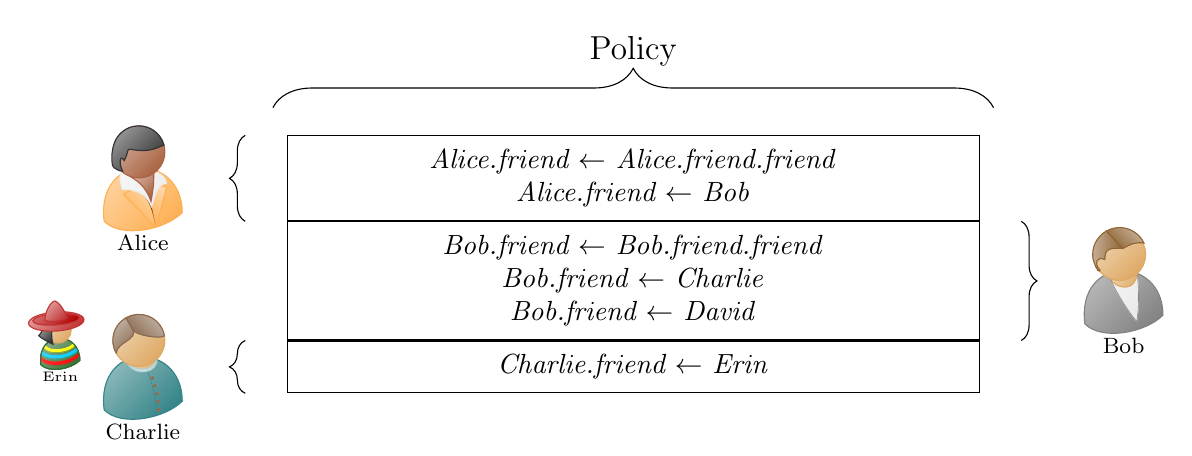
\begin{tikzpicture}
        \tikzstyle{credential}=[rectangle, draw, minimum width=250];
        
        \node [credential] (A) {\begin{tabular}{c}
            \textit{Alice.friend $\gets$ Alice.friend.friend} \\
            \textit{Alice.friend $\gets$ Bob}   
        \end{tabular}};
        \node [credential, below=0 of A] (B) {\begin{tabular}{c}
            \textit{Bob.friend $\gets$ Bob.friend.friend} \\
            \textit{Bob.friend $\gets$ Charlie} \\
            \textit{Bob.friend $\gets$ David}   \\
        \end{tabular}};
        \node [credential, below=0 of B] (C) {\begin{tabular}{c}
            \textit{Charlie.friend $\gets$ Erin}
        \end{tabular}};
    
        \draw [decorate, decoration={brace, amplitude=0.5cm}] ([yshift=10pt, xshift=-5pt] A.north west) -- ([yshift=10pt, xshift=5pt] A.north east) node [black, midway, above=0.4cm, font=\large] {Policy};
    
        \draw [decorate, decoration={brace, amplitude=0.2cm, mirror}] ([xshift=-15pt] A.north west) -- ([xshift=-15pt] A.south west) node [midway, left=0.8cm, alice, minimum size=1cm, font=\footnotesize] (Alice) {Alice};
        
        \draw [decorate, decoration={brace, amplitude=0.2cm}] ([xshift=15pt] B.north east) -- ([xshift=15pt] B.south east) node [midway, right=0.8cm, bob, minimum size=1cm, font=\footnotesize] (Bob) {Bob};
        
        \draw [decorate, decoration={brace, amplitude=0.2cm, mirror}] ([xshift=-15pt] C.north west) -- ([xshift=-15pt] C.south west) node [midway, left=0.8cm, charlie, minimum size=1cm, font=\footnotesize] (Charlie) {Charlie};
        
        \node[mexican , minimum size=0.5cm, left=0.3cm of Charlie, yshift=0.3cm, font=\tiny] (Erin) {Erin};
    \end{tikzpicture}}
\end{frame}
\fi

\begin{frame}{CAM protocol}
	\centering \includegraphics[width=0.9\linewidth]{pic/prot1.png}
	*$C_{MN} \equiv CNA$
	\begin{block}{Initial state assumptions}
		\begin{itemize}
			\item \textbf{A11}: $CN \xtext{believes} ADP(CGAP_{MN}, HoA, PU_{MN})$
			\item \textbf{A12}: $CN \xtext{believes} SV(\lfloor BU\rfloor_{PU_{MN}^{-1}}, PU_{MN}, BU)$\footnote{BU will be defined in the Interpretation step}
			\item \textbf{A13}: $CN \xtext{believes} fresh(ts)$
		\end{itemize}
	\end{block}
\end{frame}
\begin{frame}{Security analysis of CAM}
	\begin{block}{Annotation}
		\begin{itemize}
			\item \textbf{A21}: $CN \xtext{received} (CoA, CNA, HoA, CGAP_{MN}, ts, S_{MN})$
		\end{itemize}
	\end{block}
	\begin{block}{Comprehension}
		\begin{itemize}
			\item \textbf{A31}: {\small $CN \xtext{believes} CN \xtext{received} (CoA, CNA,HoA,\langle CGAP_{MN}\rangle_{*CN},ts, \left\langle S_{MN}\right\rangle_{*CN})$}
		\end{itemize}
	\end{block}
	\begin{block}{Interpretation}
		\begin{itemize}
			\item \textbf{A41}: {\small $CN \xtext{believes} CN \xtext{received} (CoA, CNA,HoA,\langle CGAP_{MN}\rangle_{*CN},ts, \left\langle S_{MN}\right\rangle_{*CN})$ \\ 
			$\rightarrow CN \xtext{believes} CN \xtext{received} (BU, \langle\lfloor BU\rfloor_{PU_{MN}^{-1}}\rangle_{*CN})$} \\ where $BU = (MN@CoA, CNA, MN@HoA, \langle CGAP_{MN}\rangle_{*CN}, ts)$
		\end{itemize}
	\end{block}
\end{frame}
\begin{frame}[label={frm:cam_derivation}]{Security analysis of CAM}
	\begin{block}{Derivation}
		\label{frm:cam1_s}
		(From A41)
		\begin{itemize}
			\item \textbf{D1}: $CN \xtext{believes} CN \xtext{received} (BU, \langle\lfloor BU\rfloor_{PU_{MN}^{-1}}\rangle_{*CN})$ \\ \hspace{1.7cm} By A31, A41 and BA1
			\item \textbf{D2}: $CN \xtext{believes} CN \xtext{received} (\langle CGAP_{MN}\rangle_{*CN} \xtext{from} MN)$ \\ \hspace{1.7cm} By D1, RA1 and BA1
			\item \textbf{D3}: $CN \xtext{believes} (KA(MN, PU_{MN}, HoA) \land PK_\sigma(MN, PU_{MN}))$ \\ \hspace{1.7cm} By D2, A11, MIP1 and BA1
			\item \textbf{D4}: $CN \xtext{believes} (OWN(MN,HoA) \land MN \xtext{said} BU)$ \\ \hspace{1.7cm} By D1, RA1, D3, A12, MIP2 and BA1
			\item \textbf{D5}: $CN \xtext{believes} MN \xtext{says} BU$ \\ \hspace{1.7cm} By D4, A13, FA1, NVA and BA1
			\item \textbf{D6}: $CN \xtext{believes} MN \xtext{says} (MN@HoA,MN@CoA)$ \\ \hspace{1.7cm} By D5, SA2 and BA1 [\underline{\ref{frm:cam1_f}}]
		\end{itemize}
	\end{block}
\end{frame}
\begin{frame}{Security analysis of CAM}
	From the previous security proof we can conclude that:
	\begin{itemize}
		\item The CAM protocol \alert{is not vulnerable to session hijacking attack}, because the MN and its public key are authenticated by the CN (D5)
		\item These beliefs cannot convince the CN that the MN indeed exists at $HoA$ and $CoA$ making the protocol vulnerable to the MMF
		\begin{itemize}
			\item $CN \xtext{believes} MN$ \textbf{says} $(MN@HoA,MN@CoA)$
			\item A malicious but legitimate $MN$ can trick its $CN$ to redirect \alert{its} traffic to a victim node
		\item The ERO protocol solves this issue
		\end{itemize}
	\end{itemize}
	\alert{Note:} this protocol can be formally verified using BAN logic without reasoning about the validity of $PU_{MN}$ ($CN \xtext{believes} MN \xtext{believes} BU$)
\end{frame}
%------------------------------
\iffalse
\begin{frame}{ERO protocol}
	\small
	\begin{center} 
		\includegraphics[width=0.7\linewidth]{pic/prot2.png}
		\vspace*{30.0cm}
		\includegraphics[width=0.7\linewidth]{pic/prot2-notation.png}
	\end{center}
\end{frame}
\fi
\begin{frame}{ERO protocol}
	\small
	\begin{columns}[T]
		\begin{column}{0.6\textwidth}
			\includegraphics[width=\linewidth]{pic/prot2.png}
		\end{column}
		\begin{column}{0.58\textwidth}
			\begin{center}
				\includegraphics[width=\linewidth]{pic/prot2-notation.png}
			\end{center}
		\end{column}
	\end{columns}
	\vspace{0.2cm}
	\begin{itemize}
		\item $HoTI, HoT$ may be performed before the $MN$ changes location
		\item $Kbmperm$ is a longterm secret used to protect the subsequent binding update messages
		\item HMAC guarantees both the integrity and authenticity of a message
		\item $MN$ shows its presence at $Hoa$ and $CoA$ proving the receipt of $Nh$ and $Nc$
		\item Once completed $CBA$, $MN$ can enter the movement phase
	\end{itemize}
\end{frame}

\iffalse
\begin{frame}{ERO protocol}
	\centering \includegraphics[width=0.9\linewidth]{pic/prot2-notation.png}
\end{frame}
\fi
\begin{frame}{Security analysis of ERO}
	\begin{block}{Initial state assumptions [1/2]}
		\begin{itemize}
			\item \textbf{A11}: $CN \xtext{believes} ADP(CGAP_{MN}, HoA, PU_{MN})$
			\item \textbf{A12}: $CN \xtext{believes} SV(\lfloor ebuBody\rfloor_{PU_{MN}^{-1}}, PU_{MN}, ebuBody)$\footnote{where $ebuBody$ is defined in the Comprehension step}
			\item \textbf{A13}: $CN \xtext{believes} fresh(Nh)$
			\item \textbf{A14}: $CN \xtext{believes} RR(Nh,MN,HoA)$
			\item \textbf{A15}: $MN \xtext{believes} ADP(CGAP_{CN},CNA,PU_{CN})$
			\item \textbf{A16}: $MN \xtext{believes} SV(\lfloor ebaBody\rfloor_{PU_{CN}^{-1}}, PU_{CN}, ebaBody)$\footnote{where $ebaBody$ is defined in the Comprehension step}
			\item \textbf{A17}: $MN \xtext{believes} fresh(Seq1)$
			\item \textbf{A18}: $MN \xtext{believes} CN \xtext{controls} St1$
		\end{itemize}
	\end{block}
\end{frame}
\begin{frame}{Security analysis of ERO}
	\begin{block}{Initial state assumptions [2/2]}
		\begin{itemize}
			\item \textbf{A19}: $MN \xtext{believes} RR(Seq1, CN, CNA)$
			\item \textbf{A1a}: $MN \xtext{believes} CN \xtext{controls} fresh(MN\xleftrightarrow{K}CN)$
			\item \textbf{A1b}: $MN \xtext{believes} PK_\psi(MN,PU_{MN})$
			\item \textbf{A1c}: $MN \xtext{believes} CN \xtext{controls} MN\xleftrightarrow{K}CN$
			\item \textbf{A1d}: $CN \xtext{believes} MN\xleftrightarrow{K2}CN$
			\item \textbf{A1e}: $CN \xtext{believes} fresh(K2)$
			\item \textbf{A1f}: $CN \xtext{believes} fresh(Nc)$
			\item \textbf{A1g}: $CN \xtext{believes} RR(Nc,MN,CoA)$
			\item \textbf{A1h}: $MN \xtext{believes} fresh(Seq2)$
			\item \textbf{A1i}: $MN \xtext{believes} CN \xtext{controls} fresh(St2)$
		\end{itemize}
	\end{block}
\end{frame}
\begin{frame}{Security analysis of ERO}	
	\begin{block}{Annotation}
		\begin{itemize}
			\item \textbf{A21}: $CN \xtext{received} (Chi)$
			\item \textbf{A22}: $MN \xtext{received} (Chi, Nh)$
			\item \textbf{A23}: $CN \xtext{received} (CoA, CNA, HoA,Seq1,Cci,Nh,CGAP_{MN}, Sebu, Mebu)$
			\item \textbf{A24}: {\small $MN \xtext{received} (CoA, CNA, HoA, Seq1,Nc,Cci,\{Kbmperm\}_{PU_{MN}},$\\\hspace{0.9cm}$CGAP_{CN}, Seba, Meba)$}
			\item \textbf{A25}: $CN \xtext{received} (CoA, CNA, HoA, Seq2,Nc,Mcbu)$
			\item \textbf{A26}: $MN \xtext{received} (CoA, CNA, St2,Seq2,Mcba)$
		\end{itemize}
	\end{block}
\end{frame}
\begin{frame}{Security analysis of ERO}
	\begin{block}{Comprehension}
		\begin{itemize}
			\item \textbf{A31}: $CN \xtext{believes} CN \xtext{received} (\langle Chi\rangle_{*CN})$
			\item \textbf{A32}: $MN \xtext{believes} MN \xtext{received} (Chi, \langle Nh\rangle_{*MN})$
			\item \textbf{A33}: $CN \xtext{believes} CN \xtext{received} (ebuBody, \langle Sebu\rangle_{*CN}, \langle Mebu\rangle_{*CN})$\\{\small where $ebuBody = (CoA, CNA, HoA, Seq1, \langle Cci\rangle_{*CN}, Nh, \langle CGAP_{MN}\rangle_{*CN} \xtext{from} MN)$}
			\item \textbf{A34}: {\small $MN \xtext{believes} MN \xtext{received} (ebaBody, \{\langle Kbmperm\rangle_{*MN}\}_{PU_{MN}},$\\$ \langle Seba\rangle_{*MN}, \langle Meba\rangle_{*MN})$ \hspace{2.0cm}where $ebaBody = (CoA, CNA, \langle St1\rangle_{*MN}, Seq1, \langle Nc\rangle_{*MN}, Cci, \langle CGAP_{CN}\rangle_{*MN} \xtext{from} CN)$}
			\item \textbf{A35}: {\small $CN \xtext{believes} CN \xtext{received} (CoA, CNA, HoA, Seq2, Nc, \langle Mcbu\rangle_{*CN})$}
			\item \textbf{A36}: {\small$MN \xtext{believes} MN \xtext{received} (CoA, CNA, \langle St2\rangle_{*MN}, Seq2, \langle Mcba\rangle_{*MN})$}
		\end{itemize}
	\end{block}
\end{frame}
\begin{frame}{Security analysis of ERO}
	\begin{block}{Interpretation}
		\begin{itemize}
			\item \textbf{A41}: (A33): {\small $CN \xtext{believes} CN \xtext{received} (ebuBody, \langle Sebu\rangle_{*CN}, \langle Mebu\rangle_{*CN})$ \\ 
			$\rightarrow CN \xtext{believes} CN \xtext{received} (ebuBody \xtext{from} MN, \langle \lfloor ebuBody\rfloor_{PU_{MN}^{-1}}\rangle_{*CN})$}
			\item \textbf{A42} (A34): {\small $MN \xtext{believes} MN \xtext{received} (ebaBody, \{\langle Kbmperm\rangle_{*MN}\}_{PU_{MN}},$ \\$ \langle Seba\rangle_{*MN},\langle Meba\rangle_{*MN})$ \\ 
			$\rightarrow MN \xtext{believes} MN \xtext{received} (\widehat{ebaBody} \xtext{from} CN, \langle \lfloor \widehat{ebaBody}\rfloor_{PU_{CN}^{-1}}\rangle_{*MN})$ \\ where $\widehat{ebaBody}=(ebaBody, \{MN \xleftrightarrow{\langle K2\rangle_{*MN}}CN\}_{PU_{MN}}, fresh(\langle K2\rangle_{*MN}))$}
			\item \textbf{A43} (A35): {\small $CN \xtext{believes} CN \xtext{received} (CoA, CNA, HoA, Seq2, Nc, \langle Mcbu\rangle_{*CN})$\\ 
			$\rightarrow CN \xtext{believes} CN \xtext{received} {+}\{(CoA, CNA, HoA, Seq2, Nc,$\\$ MN \xleftrightarrow{K2}CN) \xtext{from} MN\}_{K2}$}
			\item \textbf{A44} (A36): {\small $MN \xtext{believes} MN \xtext{received} (CoA, CNA, St2, Seq2, \langle Mcba\rangle_{*MN}) \rightarrow $\\ 
			$MN \xtext{believes} MN \xtext{received} {+}\{(CoA, CNA, \langle St2\rangle_{*MN},Seq2) \xtext{from} CN\}_{\langle K2\rangle_{*MN}}$}
		\end{itemize}
	\end{block}
\end{frame}
\begin{frame}{Security analysis of ERO}
	\begin{block}{Derivation [1/4]}
		\label{frm:ero1_s}
		\small
		(From A41)
		\vspace{-0.2cm}
		\begin{itemize}
			\item \textbf{D1}: {\small $CN \xtext{believes} CN \xtext{received} (ebuBody \xtext{from} MN, \langle \lfloor ebuBody\rfloor_{PU_{MN}^{-1}}\rangle_{*CN})$ \\ \hspace{1.7cm} By A33, A41 and BA1}
			\item \textbf{D2}: $CN \xtext{believes} CN \xtext{received} (\langle CGAP_{MN}\rangle_{*CN} \xtext{from} MN)$ \\ \hspace{1.7cm} By D1, RA1 and BA1
		\end{itemize}
		... applying the same rules as the CAM Derivation on slide \ref{frm:cam_derivation} we obtain:
		\begin{itemize}
			\item \textbf{D4}: $CN \xtext{believes} (OWN(MN,HoA) \land MN \xtext{said} ebuBody)$
			\item \textbf{D5}: $CN \xtext{believes} MN \xtext{says} ebuBody$
			\item \textbf{D6}: $CN \xtext{believes} MN \xtext{says} (HoA, CoA)$ \\ \hspace{1.7cm} By D5, SA2 and BA1
			\item \textbf{D7}: $CN \xtext{believes} MN@HoA$ \\ \hspace{1.7cm} By D5, SA2, A14, MIP4 and BA1 [\underline{\ref{frm:ero1_f}}]
		\end{itemize}
		\vspace{-0.2cm}
		that verifies the first part.
	\end{block}
\end{frame}
\begin{frame}{Security analysis of ERO}
	\begin{block}{Derivation [2/4]}
		(From A42)
		\begin{itemize}
			\item \textbf{D8}: {\small $MN \xtext{believes} MN \xtext{received} (\widehat{ebaBody} \xtext{from} CN, \langle \lfloor \widehat{ebaBody}\rfloor_{PU_{CN}^{-1}}\rangle_{*MN})$ \\ \hspace{1.7cm} By A34, A42 and BA1}
			\item \textbf{D9}: {\small $MN \xtext{believes} MN \xtext{received} (KA(CN,PU_{CN}, CNA) \land PK_\sigma(CN, PU_{CN}))$ \\ \hspace{1.7cm} By D8, RA1, A15, MIP1 and BA1}
			\item \textbf{D10}: {\small $MN \xtext{believes} (MN \xtext{received} OWN(CN,CNA) \land CN \xtext{said} \widehat{ebaBody})$ \\ \hspace{1.7cm} By D8, RA1, D9, A16, MIP2 and BA1}
			\item \textbf{D11}: {\small $MN \xtext{believes} CN \xtext{says} \widehat{ebaBody}$ \\ \hspace{1.7cm} By D10, A17, FA1, NVA and BA1}
			\item \textbf{D12}: {\small $MN \xtext{believes} \langle St1\rangle_{*MN}$ \\ \hspace{1.7cm} By D11, SA2, A18, JA and BA1}
		\end{itemize}
	\end{block}
\end{frame}
\begin{frame}{Security analysis of ERO}
	\begin{block}{Derivation [2/4]}
		\label{frm:ero2_s}
		\vspace{0.4cm}...
		\begin{itemize}
			\item \textbf{D13}: {\small $MN \xtext{believes} CN@CNA$ \\ \hspace{1.7cm} By D11, SA2, A19, MIP4 and BA1}
			\item \textbf{D14}: {\small $MN \xtext{believes} fresh(\langle K2\rangle_{*MN})$ \\ \hspace{1.7cm} By D11, SA2, A1a, JA and BA1}
			\item \textbf{D15}: {\small $MN \xtext{believes} MN \xleftrightarrow{\langle K2\rangle_{*CN}} CN$ \\ \hspace{1.7cm} By D10, SA1, A1b, SA3, D14, NVA, A1c, JA and BA1 [\underline{\ref{frm:ero2_f}}]}
		\end{itemize}
		that verifies the second part.
	\end{block}
\end{frame}
\begin{frame}{Security analysis of ERO}
	\begin{block}{Derivation [3/4]}
		(From A43)
		\begin{itemize}
			\item \textbf{D16}: {\small $CN \xtext{believes} CN \xtext{received} {+}\{(CoA, CNA, HoA, Seq2, Nc, MN \xleftrightarrow{K2}CN) \xtext{from} MN\}_{K2}$ \\ \hspace{1.7cm} By A35, A43 and BA1}
			\item \textbf{D17}: {\small $CN \xtext{believes} MN \xtext{said} (CoA, CNA, HoA, Seq2, Nc, MN \xleftrightarrow{K2} CN)$ \\ \hspace{1.7cm} By A1d, D16, SAA3 and BA1}
			\item \textbf{D18}: {\small $CN \xtext{believes} MN \xtext{says} (CoA, CNA, HoA, Seq2, Nc, MN \xleftrightarrow{K2} CN)$ \\ \hspace{1.7cm} By A1f, D17, FA1, NVA and BA1}
			\item \textbf{D19}: {\small $CN \xtext{believes} MN \xtext{says} MN \xleftrightarrow{K2} CN$ \\ \hspace{1.7cm} By D18, SA2 and BA1}
			\item \textbf{D20}: {\small $CN \xtext{believes} MN@CoA$ \\ \hspace{1.7cm} By D18, SA2, A1g, MIP4 and BA1}
		\end{itemize}
		\par that verifies the third part.
	\end{block}
\end{frame}
\begin{frame}{Security analysis of ERO}
	\begin{itemize}
		\item D19 guarantees that the $CN$ belief to successfully share $K2$ with the $MN$
		\item D20 shows that the $CN$ trusts the $MN$ exists at $CoA$. In other words, \alert{the ERO protocol is not vulnerable to the MMF attack anymore}
	\end{itemize}
\end{frame}
\begin{frame}{Security analysis of ERO}
	\begin{block}{Derivation [4/4]}
		(From A44)
		\begin{itemize}
			\item \textbf{D21}: {\small $MN \xtext{believes} MN \xtext{received} {+}\{(CoA, CNA, \langle St2\rangle_{*MN}, Seq2) \xtext{from} MN\}_{\langle K2\rangle_{*MN}}$ \\ \hspace{1.7cm} By A36, A44 and BA1}
			\item \textbf{D22}: {\small $MN \xtext{believes} CN \xtext{said} (CoA, CNA, \langle St2\rangle_{*MN}, Seq2)$ \\ \hspace{1.7cm} By D15, D21, SAA3 and BA1}
			\item \textbf{D23}: {\small $MN \xtext{believes} CN \xtext{says} (CoA, CNA, \langle St2\rangle_{*MN}, Seq2)$ \\ \hspace{1.7cm} By A1h, D22, FA1, NVA and BA1}
			\item \textbf{D24}: {\small $MN \xtext{believes} \langle St2\rangle_{*MN}$ \\ \hspace{1.7cm} By D23, A1i, JA and BA1}
		\end{itemize}
		\par that ends the proof.
	\end{block}
\end{frame}
\begin{frame}{Security analysis of ERO}
	From the formal analysis we obtain the following results:
	\begin{itemize}
		\item The $CN$ believes the $MN$ owns $HoA$ while being at $HoA$ and $CoA$. So, the protocol \alert{can prevent the redirect attacks} (D4, D7, D20)
		\item $K2$ is a good key shared between the $CN$ and the $MN$ (D14, D15, D19, A1d, A1e)
	\end{itemize}
\end{frame}
%%%%%%%%%%%%%%%%%%%%%%%%%%%%%%%%%%%%%%
\section{Conclusions}
\begin{frame}{Conclusions}
   \begin{itemize}
	   \item A brief introduction about the motivations behind the SVO logic was made. Subsequently, the notation and constructs of SVO were observed, showing that SVO is more than an extension of BAN logic
	   \item We introduced the MIPv6 as the (not so) future standard for mobile communications, showing its architecture and security concerns
	   \item Finally, we gave a formal verification of the MIPv6 security protocols using SVO logic, in particular proving that the CAM protocol is vulnerable to MMF attacks while the ERO protocol is not
   \end{itemize}
\end{frame}

\begin{frame}[standout]
	Questions?
\end{frame}
  
\appendix
%%%%%%%%%%%%%%%%%%%%%%%%%%%%%%%%%%%%%%
\begin{frame}{References}
	\small
	\begin{itemize}
		\item Syverson, Paul F., and Paul C. Van Oorschot. "On unifying some cryptographic protocol logics." \textit{Proceedings of 1994 IEEE Computer Society Symposium on Research in Security and Privacy.} IEEE, 1994.
		\item Syverson, Paul, and Iliano Cervesato. "The logic of authentication protocols." \textit{International School on Foundations of Security Analysis and Design.} Springer, Berlin, Heidelberg, 2000.
		\item Kuang, Shilei, Robert Elz, and Sinchai Kamolphiwong. "Investigating enhanced route optimization for mobile IPv6." 2008 \textit{13th Asia-Pacific Computer Systems Architecture Conference.} IEEE, 2008.
		\item You, Ilsun, Yoshiaki Hori, and Kouichi Sakurai. "Enhancing SVO Logic for Mobile IPv6 Security Protocols." \textit{J. Wirel. Mob. Networks Ubiquitous Comput. Dependable Appl.} 2.3 (2011): 26-52.
		\item Stefano Chessa's notes for the Mobile and CyberPhysical Systems course.
		\item Kurose, James F., and Keith W. Ross. "Computer Networking: A Top-Down Approach . 6th." Harlow, UK: Pearson Education Ltd (2012).
	\end{itemize}
\end{frame}

\begin{frame}[standout]
\end{frame}
\begin{frame}
	\label{frm:cam1_f}
	\begin{itemize}
		\item [] \textbf{D4}: $CN \xtext{believes} (OWN(MN,HoA) \land MN \xtext{said} BU)$
		\item [$\implies$] (A13) $CN \xtext{believes} (MN \xtext{said} BU \land fresh(ts))$
		\item [$\implies$] (FA1) $CN \xtext{believes} (MN \xtext{said} BU \land fresh(BU))$
		\item [$\implies$] (NVA) $(MN \xtext{said} BU \land fresh(BU)) \rightarrow MN \xtext{says} BU$
		\item [] \textbf{D5}: $CN \xtext{believes} MN \xtext{says} BU$ \\ \hspace{1.7cm} By D4, A13, FA1, NVA and BA1
	\end{itemize}
	[\underline{\ref{frm:cam1_s}}]
\end{frame}
\begin{frame}
	\label{frm:ero1_f}
	\begin{itemize}
		\item [] \textbf{D5}: $CN \xtext{believes} MN \xtext{says} ebuBody$
		\item [$\implies$] (SA2) $CN \xtext{believes} MN \xtext{says} Nh$
		\item [$\implies$] (A14) $CN \xtext{believes} (MN \xtext{says} Nh \land RR(Nh,MN,HoA))$
		\item [$\implies$] (MIP4) $(MN \xtext{says} Nh \land RR(Nh,MN,HoA))\rightarrow MN@HoA$
		\item [] \textbf{D7}: $CN \xtext{believes} MN@HoA$ \\ \hspace{1.7cm} By D5, SA2, A14, MIP4 and BA1
	\end{itemize}
	[\underline{\ref{frm:ero1_s}}]
\end{frame}
\begin{frame}
	\label{frm:ero2_f}
	\small
	\begin{itemize}
		\item [] \textbf{D10}: $MN \xtext{believes} (MN \xtext{received} OWN(CN,CNA) \land CN \xtext{said} \widehat{ebaBody})$
		\item [$\implies$] (SA1) $MN \xtext{believes} CN \xtext{said} \{MN \xleftrightarrow{\langle K2\rangle_{*MN}}CN\}_{PU_{MN}}$
		\item [$\implies$] (A1b) $MN \xtext{believes} (CN \xtext{said} \{MN \xleftrightarrow{\langle K2\rangle_{*MN}}CN\}_{PU_{MN}} \land PK_\psi(MN, PU_{MN}))$
		\item [$\implies$] (SA3) $((CN \xtext{said} \{MN \xleftrightarrow{\langle K2\rangle_{*MN}}CN\}_{PU_{MN}}) \land (PK_\psi(MN, PU_{MN}))$ \\$ \rightarrow (CN \xtext{said} MN \xleftrightarrow{\langle K2\rangle_{*MN}}CN)$
		\item [$\implies$] (D14) $MN \xtext{believes} (fresh(\langle K2\rangle_{*MN}) \land (CN \xtext{said} MN \xleftrightarrow{\langle K2\rangle_{*MN}}CN))$
		\item [$\implies$] (NVA) $(fresh(\langle K2\rangle_{*MN}) \land (CN \xtext{said} MN \xleftrightarrow{\langle K2\rangle_{*MN}}CN)) $ \\ $\rightarrow (CN \xtext{says} MN \xleftrightarrow{\langle K2\rangle_{*MN}}CN)$
		\item [$\implies$] (A1c) $MN \xtext{believes} ((CN \xtext{controls} MN\xleftrightarrow{K}CN) \land (CN \xtext{says} MN \xleftrightarrow{\langle K2\rangle_{*MN}}CN))$
		\item [$\implies$] (JA) $((CN \xtext{controls} MN\xleftrightarrow{K}CN) \land (CN \xtext{says} MN \xleftrightarrow{\langle K2\rangle_{*MN}}CN))$ \\$\rightarrow (MN \xleftrightarrow{\langle K2\rangle_{*CN}} CN)$
		\item [] \textbf{D15}: {\small $MN \xtext{believes} MN \xleftrightarrow{\langle K2\rangle_{*CN}} CN$ \\ \hspace{1.7cm} By D10, SA1, A1b, SA3, D14, NVA, A1c, JA and BA1}
	\end{itemize}
	[\underline{\ref{frm:ero2_s}}]
\end{frame}
\begin{frame}{ERO protocol}
	
	\begin{center} 
		\includegraphics[width=0.7\linewidth]{pic/prot2.png}
		\vspace*{30.0cm}
		\includegraphics[width=0.7\linewidth]{pic/prot2-notation.png}
	\end{center}
\end{frame}
\end{document}